\def \serialnumtrials {5}
\def \serialblocksize {64}
\def \serialtable {
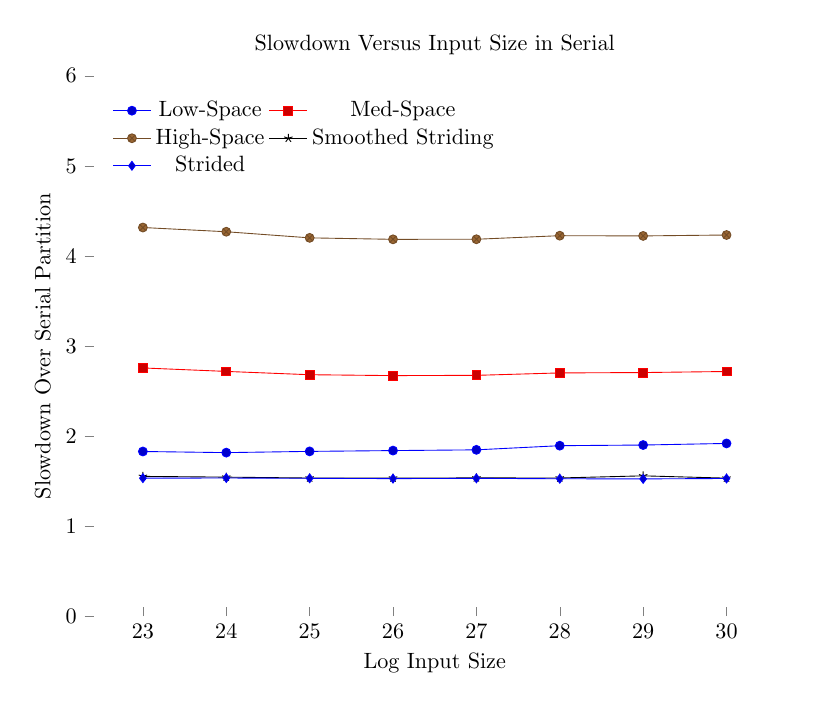
\begin{tikzpicture}[scale = .8]
\begin{axis}[
width = 5 in,
height = 4in,
title={Slowdown Versus Input Size in Serial},
xtick pos=left,
ytick pos=left,
ymax = 6,
ymin = 0,
legend style={draw=none},
axis line style = { draw = none },
legend pos= north west,
xtick = data,
xlabel={Log Input Size},
ylabel={Slowdown Over Serial Partition},
legend columns = 2,
scatter/classes=%
{a={mark=o,draw=blue}}]
%% Serial Baseline
%% baselines in ms: \addplot coordinates {( 23, 30.4 ) ( 24, 61 ) ( 25, 122.4 ) ( 26, 244.8 ) ( 27, 489.6 ) ( 28, 979.6 ) ( 29, 1963.4 ) ( 30, 3922.6 ) };
%% In-Place
\addplot coordinates {( 23, 1.82895) ( 24, 1.81639) ( 25, 1.83007) ( 26, 1.83905) ( 27, 1.84722) ( 28, 1.89343) ( 29, 1.90068) ( 30, 1.91837) };
%% In-Place Prefix-Sum
\addplot coordinates {( 23, 2.75658) ( 24, 2.71803) ( 25, 2.68137) ( 26, 2.67157) ( 27, 2.67443) ( 28, 2.70131) ( 29, 2.70551) ( 30, 2.71713) };
%% Out-of-Place
\addplot coordinates {( 23, 4.31579) ( 24, 4.26885) ( 25, 4.20098) ( 26, 4.18464) ( 27, 4.18546) ( 28, 4.22519) ( 29, 4.22257) ( 30, 4.23265) };
%% %% High-Span
%% \addplot coordinates {( 23, 1.23684) ( 24, 1.23934) ( 25, 1.24346) ( 26, 1.24428) ( 27, 1.24632) ( 28, 1.24602) ( 29, 1.24417) ( 30, 1.2456) };
%% Cache-Friendly
\addplot coordinates {( 23, 1.55263) ( 24, 1.54426) ( 25, 1.53431) ( 26, 1.53431) ( 27, 1.53554) ( 28, 1.53491) ( 29, 1.55852) ( 30, 1.53317) };
%% Strided
\addplot coordinates {( 23, 1.53289) ( 24, 1.53443) ( 25, 1.53105) ( 26, 1.52778) ( 27, 1.53064) ( 28, 1.52613) ( 29, 1.5246) ( 30, 1.52919) };
\legend{Low-Space, Med-Space, High-Space, Smoothed Striding, Strided}
\end{axis}
\end{tikzpicture}
}
%% \def \serialnumtrials {5}
%% \def \serialblocksize {64}
%% \def \serialtable {
%% \begin{tikzpicture}[scale = .8]
%% \begin{axis}[
%% width = 5 in,
%% height = 4in,
%% title={Slowdown Versus Input Size in Serial},
%% xtick pos=left,
%% ytick pos=left,
%% ymax = 5,
%% ymin = 0,
%% legend style={draw=none},
%% axis line style = { draw = none },
%% legend pos= north west,
%% xtick = data,
%% xlabel={Log Input Size},
%% ylabel={Slowdown Over Serial Partition},
%% legend columns = 2,
%% scatter/classes=%
%% {a={mark=o,draw=blue}}]
%% %% Serial Baseline
%% %% baselines in ms: \addplot coordinates {( 23, 30.4 ) ( 24, 61 ) ( 25, 122.4 ) ( 26, 244.8 ) ( 27, 489.6 ) ( 28, 979.6 ) ( 29, 1963.4 ) ( 30, 3922.6 ) };
%% %% In-Place
%% \addplot coordinates {( 23, 1.82895) ( 24, 1.81639) ( 25, 1.83007) ( 26, 1.83905) ( 27, 1.84722) ( 28, 1.89343) ( 29, 1.90068) ( 30, 1.91837) };
%% %% In-Place Prefix-Sum
%% \addplot coordinates {( 23, 2.75658) ( 24, 2.71803) ( 25, 2.68137) ( 26, 2.67157) ( 27, 2.67443) ( 28, 2.70131) ( 29, 2.70551) ( 30, 2.71713) };
%% %% Out-of-Place
%% \addplot coordinates {( 23, 4.31579) ( 24, 4.26885) ( 25, 4.20098) ( 26, 4.18464) ( 27, 4.18546) ( 28, 4.22519) ( 29, 4.22257) ( 30, 4.23265) };
%% %% High-Span
%% \addplot coordinates {( 23, 1.23684) ( 24, 1.23934) ( 25, 1.24346) ( 26, 1.24428) ( 27, 1.24632) ( 28, 1.24602) ( 29, 1.24417) ( 30, 1.2456) };
%% %% Cache-Friendly
%% \addplot coordinates {( 23, 1.55263) ( 24, 1.54426) ( 25, 1.53431) ( 26, 1.53431) ( 27, 1.53554) ( 28, 1.53491) ( 29, 1.55852) ( 30, 1.53317) };
%% %% Strided
%% \addplot coordinates {( 23, 1.53289) ( 24, 1.53443) ( 25, 1.53105) ( 26, 1.52778) ( 27, 1.53064) ( 28, 1.52613) ( 29, 1.5246) ( 30, 1.52919) };
%% \legend{Low-Space, Med-Space, High-Space, Two-Layer, Cache-Friendly, Strided}
%% \end{axis}
%% \end{tikzpicture}
%% }
%% \def \serialnumtrials {1}
%% \def \serialblocksize {64}
%% \def \serialtable {
%% \begin{tikzpicture}[scale = .8]
%% \begin{axis}[
%% title={Slowdown Versus Input Size in Serial},
%% width = 5in, %%!!!!
%% height = 4in,
%% xtick pos=left,
%% ytick pos=left,
%% ymax = 5, %% !!!
%% ymin = 0,
%% legend style={draw=none},
%% axis line style = { draw = none },
%% legend pos= north west,
%% xtick = data,
%% xlabel={Log Input Size},
%% ylabel={Slowdown Over Serial Partition},
%% legend columns = 2,
%% scatter/classes=%
%% {a={mark=o,draw=blue}}]
%% %% Serial Baseline%% baselines in ms: \addplot coordinates {( 23, 30.4 ) ( 24, 60.8 ) ( 25, 121.4 ) ( 26, 243.8 ) ( 27, 487.4 ) ( 28, 975.8 ) ( 29, 1952.2 ) ( 30, 3902 ) };
%% %% In-Place
%% \addplot coordinates {( 23, 1.79605) ( 24, 1.82237) ( 25, 1.84185) ( 26, 1.84249) ( 27, 1.87033) ( 28, 1.90838) ( 29, 1.90687) ( 30, 1.91579) };
%% %% In-Place Prefix-Sum
%% \addplot coordinates {( 23, 2.58553) ( 24, 2.57237) ( 25, 2.57661) ( 26, 2.56932) ( 27, 2.56422) ( 28, 2.59459) ( 29, 2.60834) ( 30, 2.61107) };
%% %% Out-of-Place
%% \addplot coordinates {( 23, 3.98684) ( 24, 3.96711) ( 25, 3.96705) ( 26, 3.96308) ( 27, 3.98195) ( 28, 4.01537) ( 29, 4.03401) ( 30, 4.06079) };
%% %% High-Span
%% \addplot coordinates {( 23, 1.21053) ( 24, 1.23355) ( 25, 1.23558) ( 26, 1.23298) ( 27, 1.23677) ( 28, 1.24124) ( 29, 1.24096) ( 30, 1.23931) };
%% \legend{Low-Space, Med-Space, High-Space, Two-Layer} %% Two-layer instead of high-span everywhere
%% \end{axis}
%% \end{tikzpicture}
%% }
%% %% Speedup on 18 threads in table of size 268435456
%% \def \serialsortspeedup {0.780189}
